\documentclass[12pt]{article}
\usepackage[T1]{fontenc}
\usepackage{float}
\usepackage{sbc-template}
\usepackage{graphicx,url}
\usepackage[brazil]{babel}   
\usepackage[utf8]{inputenc}  
\usepackage{indentfirst}
\usepackage{caption3}
\usepackage{color}
\usepackage{alltt}
\usepackage{url}
\usepackage{listings}

\lstset{ %
language=C,                % choose the language of the code
basicstyle=\footnotesize,       % the size of the fonts that are used for the code
numbers=left,                   % where to put the line-numbers
numberstyle=\footnotesize,      % the size of the fonts that are used for the line-numbers
stepnumber=1,                   % the step between two line-numbers. If it is 1 each line will be numbered
numbersep=7pt,                  % how far the line-numbers are from the code
backgroundcolor=\color{white},  % choose the background color. You must add \usepackage{color}
showspaces=false,               % show spaces adding particular underscores
showstringspaces=false,         % underline spaces within strings
showtabs=false,                 % show tabs within strings adding particular underscores
frame=single,           % adds a frame around the code
tabsize=2,          % sets default tabsize to 2 spaces
breaklines=true,        % sets automatic line breaking
breakatwhitespace=false,    % sets if automatic breaks should only happen at whitespace
escapeinside={\%*}{*)},          % if you want to add a comment within your code
extendedchars=true,
emph={%  
    set, pair, bool%
    },emphstyle={\bfseries},
morekeywords={set, pair}
literate={á}{{\'a}}1 {ã}{{\~a}}1 {é}{{\'e}}1
}
     
\sloppy

\title{siC: Uma linguagem baseada em C incluindo pilha e fila como tipos primitivos}

\author{Gabriella de Oliveira Esteves, 110118995}

\address{Departamento de Ciência da Computação - Universidade de Brasília}

\begin{document} 

\maketitle

%------------------------------------------------
\section{Objetivo}

Este trabalho visa projetar e construir uma nova linguagem chamada de siC - Structures in C, baseada na linguagem C. O siC acrescenta três estruturas de dados, pilha e fila, como tipos de dados primitivos e, para manipulá-las, adiciona certas operações próprias para tal.

%------------------------------------------------
\section{Introdução}

\indent Um compilador é um programa que recebe como entraga um código fonte e o traduz para um programa equilavente em outra linguagem \cite{book}. Ele pode ser dividido em sete fases, ilustrado na Figura \ref{fig:compilador}.

\begin{figure}[!ht]
  \centering
  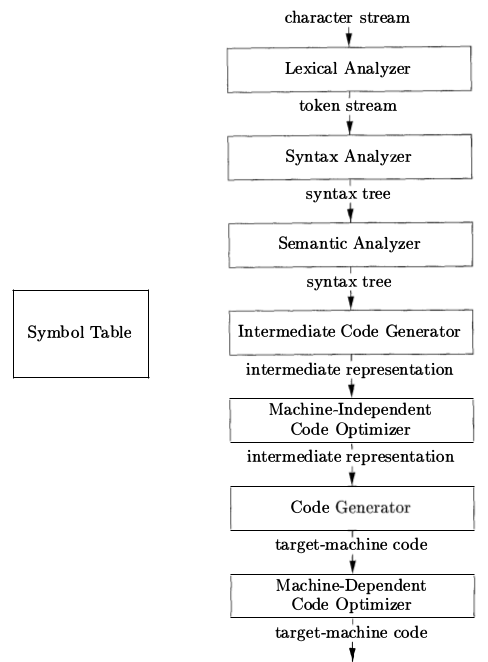
\includegraphics[width=0.5\textwidth]{compilador.png}
  \caption{Fases de um compilador} \label{fig:compilador}
\end{figure}

\begin{itemize}
	\item[1] \textbf{Analisador Léxico:} Lê o código fonte e atribui significado à cada sequência de caracteres, agora chamados lexemas. Cada lexema é mapeado para um token, que por sua vez é um par de nome (símbolo abstrato) e atributo (ponteiro para tabela de símbolos);
	\item[2] \textbf{Analisador Sintático:} Constrói uma representação gramátical dos tokens em forma de árvore;
	\item[3] \textbf{Analisador Semântico:} Utiliza a árvore sintática juntamente com a tabela de símbolos para verificar se a consistência semântica é mantida de acordo com a definição da linguagem.
	\item[4] \textbf{Gerador de Código Intermediário:} Converte árvore sintática anotada em código intermediário, com linguagem parecida com assembly e que possui apenas três operadores por linha de código. Nesse sentido, quebra-se estruturas complexas em estruturas mais simples, nesta fase.
	\item[5, 6] \textbf{Otimizador de Código Independente/Dependente de Máquina:} Procura aprimorar o código intermediário com o objetivo de melhorar o código-alvo de alguma forma: o deixando mais rápido, mais curto, consumindo menos energia, etc.
	\item[7] \textbf{Gerador de Código:} Converte o código intermediário no código-alvo, 	buscando atribuir os registradores às variáveis da maneira ótima.
\end{itemize}

\indent O foco do projeto será nas fase 1, 2, 3 e 4, porém a princípio serão apresentadas apenas a descrição da linguagem siC, bem como uma breve descrição de sua semântica. Como pilha e fila são duas das estruturas de dados mais básicas, é possível dizer que siC se destina a inúmeras áreas de Ciência da Computação, como sistemas operacionais (onde a fila é usada para organizar prioridades dos processos, por exemplo), compiladores (onde a pilha é usada para ordenar a execução dos métodos/funções), etc.

\indent Dois grandes motivos sustentam a escolha do tema deste projeto. Primeiro, uma vez que as estruturas de dados pilha e fila fazem parte dos tipos primitivos de uma linguagem, haverá menos manipulação de ponteiros na mesma, portanto erros envolvendo-os são menos prováveis de ocorrer. Segundo, a linguagem siC é mais alto-nível que C devido à abstração das estruturas de dados báscias, e, de maneira geral, pode ser mais \textit{user-friendly}. Nesse sentido, o usuário (da linguagem) leigo deverá entender como cada estrutura funciona, bem como suas vantagens/desvantagens e usabilidade; porém a implementação de cada uma estará a cargo da própria siC. 

\section{Gramática}

\indent A seguir será apresentada a gramática da linguagem siC, baseada em C \cite{yacc}. Alguns comentários são feitos ao longo da gramática para facilitar o entendimento das variáveis e nomenclatura utilizada. As palavras reservadas da linguagen são representadas aqui como \textit{tokens}. As variáveis e constantes são representadas como \textit{identifiers}, que por sua vez é uma expressão regular, e a única diferença entre este e \textit{identifier\_struct} é que o segundo tem acesso ao topo da pilha ou início da fila caso estes sejam os tipos do \textit{identifier}. Segue abaixo a gramática proposta, em que a variável inicial é \textit{function}.

\begin{alltt}{\footnotesize

token: WHILE, IF, ELSE, RETURN, STACK, TOP, QUEUE, FIRST, VOID, BOOL, INT, CHAR

function
   \(\to\) type identifier `(' argument `)' `\{' statement `RETURN' identifier `;' `\}'
    | type identifier `(' `)' `\{' statement `\}'
    
identifier
   \(\to\) letra(letra | digito)*
    
letra
   \(\to\) `a' | `b' | \dots | `z'
    
digito
   \(\to\) `0' | `1' | \dots | `9'
	
identifier\_struct
   \(\to\) identifier
    | \textbf{identifier `.' TOP}
    | \textbf{identifier `.' FIRST}	
	
type\_struct
   \(\to\) type\_simple
    | \textbf{type\_stack}
    | \textbf{type\_queue}
    
type\_simple
   \(\to\) VOID
    | BOOL
    | INT
    | CHAR
   
}\end{alltt}
\indent Existem dois novos tipos de dados, \textit{STACK} e \textit{QUEUE}, que serão compostas por tipos simples de dados apenas (ou seja, não será possível criar uma variável do tipo pilha onde seus elementos também são pilhas). Caso a variável seja do tipo pilha, ela poderá obter o topo através do comando "identifier.TOP". Caso seja fila, poderá obter o primeiro elemento com "identifier.FIRST".

\begin{alltt}{\footnotesize      
\textbf{
type\_stack
   \(\to\) STACK `<' type\_simple `>'

type\_queue
   \(\to\) QUEUE `<' type\_simple `>'
}

argument
   \(\to\) type\_struct identifier
    | type\_struct identifier `,' type\_struct identifier

}\end{alltt}
\indent A seguir serão descritas quatro estruturas básicas da linguagem siC: comando com repetição, condicional, expressões matemáticas e expressões com pilhas e filas. A última contempla as operações de adicionar elemento no topo da pilha ou no fim da fila, "+", e remover do topo ou do início da fila, "-", onde o valor do elemento retirado é armazenado no último operando da expressão.

\begin{alltt}{\footnotesize
statement
   \(\to\) declare\_identifier
    | while\_expression
    | if\_expression
    | math\_expression
    | \textbf{identifier\_struct\_expression}
    | \(\varepsilon\)
		
declare\_identifier
   \(\to\) argument ';' 
		
while\_expression
   \(\to\) WHILE `(' compare\_expression `)' `\{' statement `\}'

if\_expression
   \(\to\) IF `(' compare\_expression `)' `\{' statement `\}'
    | IF `(' compare\_expression `)' `\{' statement `\}' ELSE `\{' statement `\}'
    
compare\_expression
   \(\to\) identifier\_struct compare\_assignment identifier\_struct
    
compare\_assignment
   \(\to\) `=='
    | `!='
    | `<='
    | `>='

math\_expression
   \(\to\) identifier `=' factor `;'

factor
   \(\to\) identifier\_struct
    | `(' number\_expression `)' 

number\_expressions
   \(\to\) number\_expression `+' term
    | number\_expression `-' term
    | term
    
term
   \(\to\) term `*' factor
    | term `/' factor
    | factor
    
\textbf{
identifier\_struct\_expression
   \(\to\) identifier `=' identifier `+' identifier `;'
    | identifier `=' identifier `-' identifier `;'
}		
}\end{alltt}

%\section{Analisador Léxico}

%\section{Analisador Sintático}

%\subsection{Árvore sintática}

%\subsection{Tabela de símbolos}

\section{Analisador Semântico}

\indent A análise semântica utiliza da árvore sintática para checar a consistência da linguagem. Uma de suas obrigações mais importantes é a checagem de tipo. No caso do siC, existem várias restrições a serem consideradas:
\begin{itemize}
    \item Para adicionar um elemento A em um identificador do tipo struct B, a atribuição deve ser do tipo B = B + A, onde A deverá ter tipo compatível com o de B;
    \item Para remover o topo/início de um identificador do tipo struct B, a atribuição deve ser do tipo B = B - A, onde A deverá ter tipo compatível com o de B;
    \item Nenhuma operação matemática (\textit{math\_expression}) pode conter um identificador do tipo pilha ou fila, apenas o topo ou início dos mesmos.
\end{itemize}


\indent Um exemplo de código em siC é aprensentado a seguir. O programa adiciona trê elementos numa pilha de inteiros e depois eles são somandos um a um e armazenados na variável \textit{sum}. Ao final, a variável \textit{lixo}, recém retirada do topo da pilha, é adicionada à \textit{sum}. Nesse sentido, o resultado final de sum deve ser 7. \\

\begin{lstlisting}[language=C]
VOID main () {
    STACK<INT> s;
    INT sum, INT lixo;

    s = s + 0;
    s = s + 1;
    s = s + 2;
    s = s + 3;    
    sum = 0;
    
    WHILE (s.TOP != 0) {    
        sum = (sum + s.TOP);
        s = s - lixo;
    }
    sum = sum + lixo;

    RETURN 0;
}

\end{lstlisting}

%\section{Geração de código intermediário}

% \section{Considerações finais}

\begin{thebibliography}{1}
\bibitem{book}
A.~V.~Abo, M.~S.~Lam, R.~Sethi, J.~D.~Ullman, \emph{Compilers - Principles, Techniques and Tools}
\hskip 1em plus
	0.5em minus 0.4em\relax 2nd ed. 1986
	
\bibitem{yacc}
ANSI C Yacc grammar, \url{http://www.quut.com/c/ANSI-C-grammar-y.html}, 18 12 2012.
\end{thebibliography}
%------------------------------------------------
\end{document}